To use geometry editor in Eclipse first thing needed to do is to create a geometry file. To create it, a new General Project should be created by $General->Project$ which is found in $File->New->Project$. Give the project some name and click finish. 
Right click the project folder $New->Other$. Find Geometry diagram from the list, the search functionality might help, choose it and click next. Refer to Figure~\ref{fig:ge-wiz-select}. Name it and click finish. On the project explorer leaf click on the file that you just generated. Geometry editor should open if it wasn't open already.

\begin{figure}[htp]
\begin{center}
  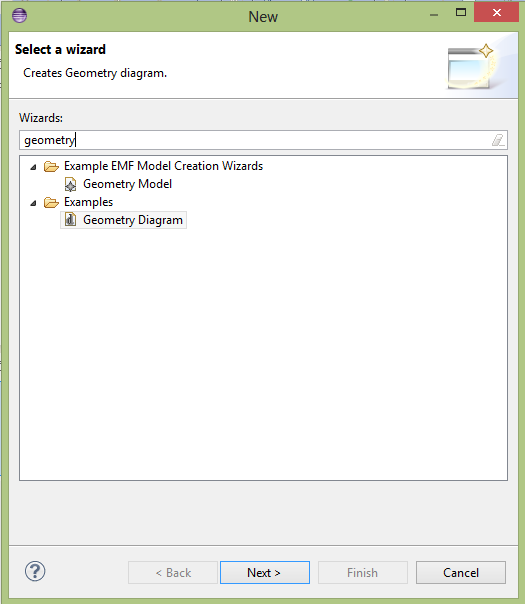
\includegraphics[width=0.8\textwidth]{image/ge-wiz-select.png}
  \caption{Select wizard for Eclipse plugins. The search functionality has been used to find geometry diagram.}
  \label{fig:ge-wiz-select}
\end{center}
\end{figure}

Figure~\ref{fig:ge-diag-empty} presents empty graphical geometry editor view. Right hand side of the view has geometry palette, which has all the available tools to be used. Rest of the view is taken by the canvas. On the geometry palette clicking InputPoint, or Connector allows user to create different points on the canvas. The points can be also created by hovering mouse on canvas and a selector tool appears after a while. InputPoint and Connector are described there by the symbols seen in geometry palette. Line tool allows drawing connections between Connectors with each other. Line can also be created by hovering mouse over a connector, which presents arrows. By clicking and dragging the arrow the new line can be thus created. BendPoints are generated by clicking a point within a line and then by dragging said point. 

\begin{figure}[htp]
\begin{center}
  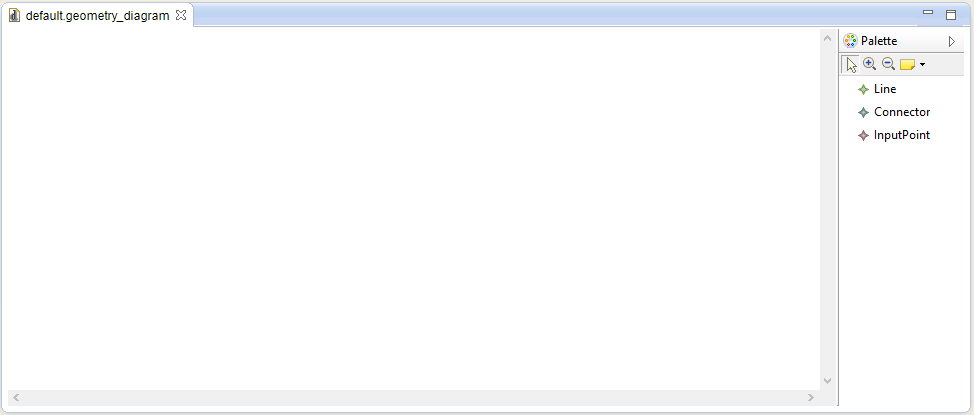
\includegraphics[width=0.8\textwidth]{image/ge-diag-empty.png}
  \caption{View of graphical geometry editor. Geometry palette can be seen on the right hand of the view and the rest is taken by canvas.}
  \label{fig:ge-diag-empty}
\end{center}
\end{figure}

Picture Figure~\ref{fig:ge-diag-exam} illustrates one example created with graphical geometry editor. InputPoints are presented by squares and Connectors are represented by circles. A geometry object line is presented by a line in the canvas. The BendPoints of a line can be seen as filled squares. However, the BendPoints are only visible when the line is selected.

\begin{figure}[htp]
\begin{center}
  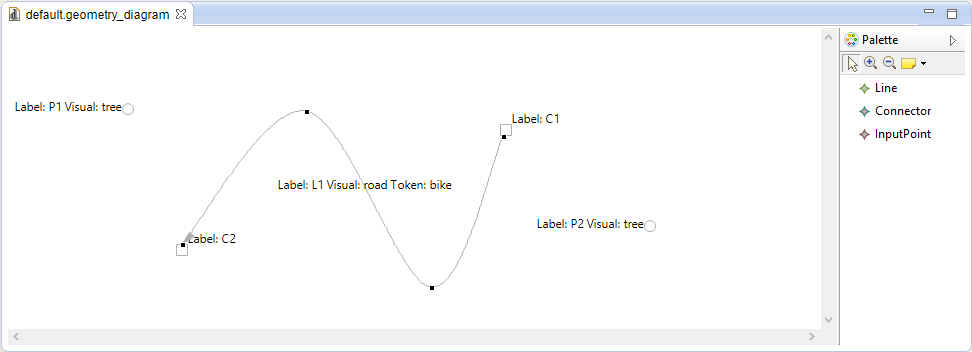
\includegraphics[width=0.8\textwidth]{image/ge-diag-exam.png}
  \caption{View of graphical geometry editor with different geometry objects.}
  \label{fig:ge-diag-exam}
\end{center}
\end{figure}

By clicking some geometry object, a property view of said object opens. If this is not visible right click on a geometry object within the canvas and click Show Properties View to open property view.
The properties view of InputPoint as seen in Figure~\ref{fig:ge-prop-input} has following properties available for editing: Appearance Label, Label, XLocation and YLocation. Appearance Label denotes to the appearance, such as a tree, a traffic light, a planet, etc, of the InputPoint within 3d simulator. Appearance Label has to have some labeling in it. Label is the name used in referring the InputPoint within the software. All the geometry objects must have different names so that references don't lead to multiple objects. XLocation and Ylocation describe coordinate location of the InputPoint. However, editing them will not change the location InputPoint in the canvas.

\begin{figure}[htp]
\begin{center}
  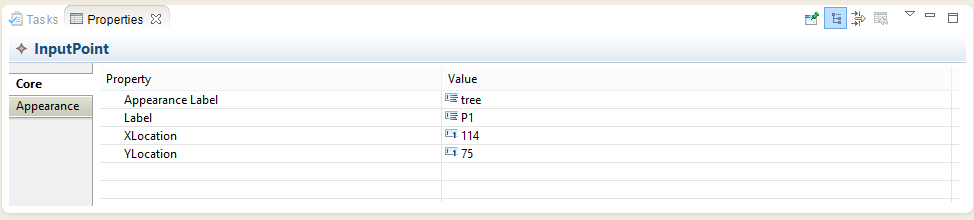
\includegraphics[width=0.8\textwidth]{image/ge-prop-input.png}
  \caption{Properties view of input point geometry object.}
  \label{fig:ge-prop-input}
\end{center}
\end{figure}

The properties view of Connector as seen in Figure~\ref{fig:ge-prop-conn} has following properties available for editing: In, Label, Out, XLocation and YLocation. In refers to the Lines that go to the Connector. And Out refers to the Lines that go from the Connector. Label is the name used in referring the Connector within the software. All the geometry objects must have different names so that references don't lead to multiple objects. XLocation and Ylocation describe coordinate location of the Connector. However, editing them will not change the location Connector in the canvas.

\begin{figure}[htp]
\begin{center}
  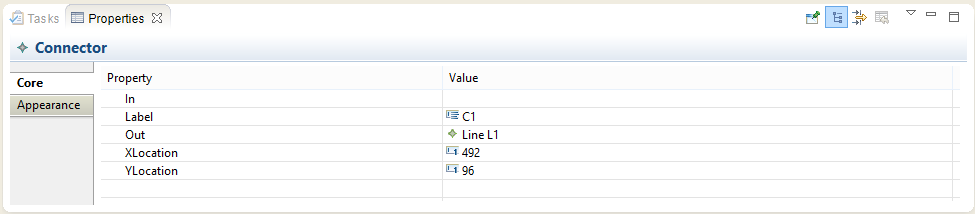
\includegraphics[width=0.8\textwidth]{image/ge-prop-conn.png}
  \caption{Properties view of connector geometry object.}
  \label{fig:ge-prop-conn}
\end{center}
\end{figure}

The properties view of Line as seen in Figure~\ref{fig:ge-prop-line} has following properties available for editing: Appearance Label, Begin, End, and Label. Appearance Label denotes to the appearance, such as a cable, a track, empty space, etc, of the Line within 3d simulator. The Appearance will extrapolated over the curve of the Line, thus creating continuous shape. Begin and End denotes the Connector of the line, which is the starting and ending point respectively of the parametric curve that is line geometry. Label is the name used in referring the Line within the software. All the geometry objects must have different names so that references don't lead to multiple objects.

\begin{figure}[htp]
\begin{center}
  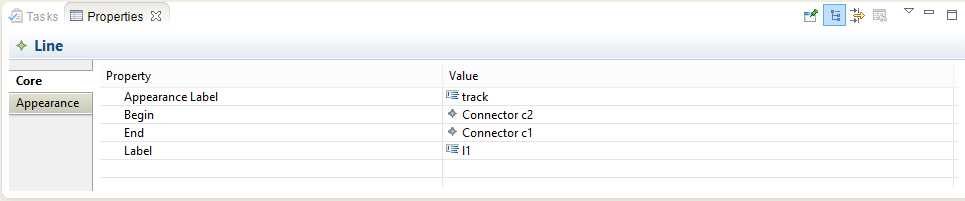
\includegraphics[width=0.8\textwidth]{image/ge-prop-line.png}
  \caption{Properties view of line geometry object.}
  \label{fig:ge-prop-line}
\end{center}
\end{figure}

